\newsection
\section{Технический проект}

\subsection{Поисковый робот}

Поисковый робот будет представлен распределенным HPC-кластером. В нем будут представлены два типа узлов:
\begin{itemize}
\item главный(master) -- узел, представленный на практике в одном экземпляре, в зону ответственности которого входит управление работой подчиненных узлов и распределение рабочей нагрузки между ними;
\item подчиненный(slave) -- узел, который выполняет однотипные порции заданий, полученных от главного узла. На практике в кластер входят несколько подчиненных узлов для эффективного распараллеливания вычислительной работы.
\end{itemize}

\subsubsection{Компоненты поискового робота}

На рисунке 3.1 представлена диаграмма компонентов поискового робота.

\begin{figure}
\center{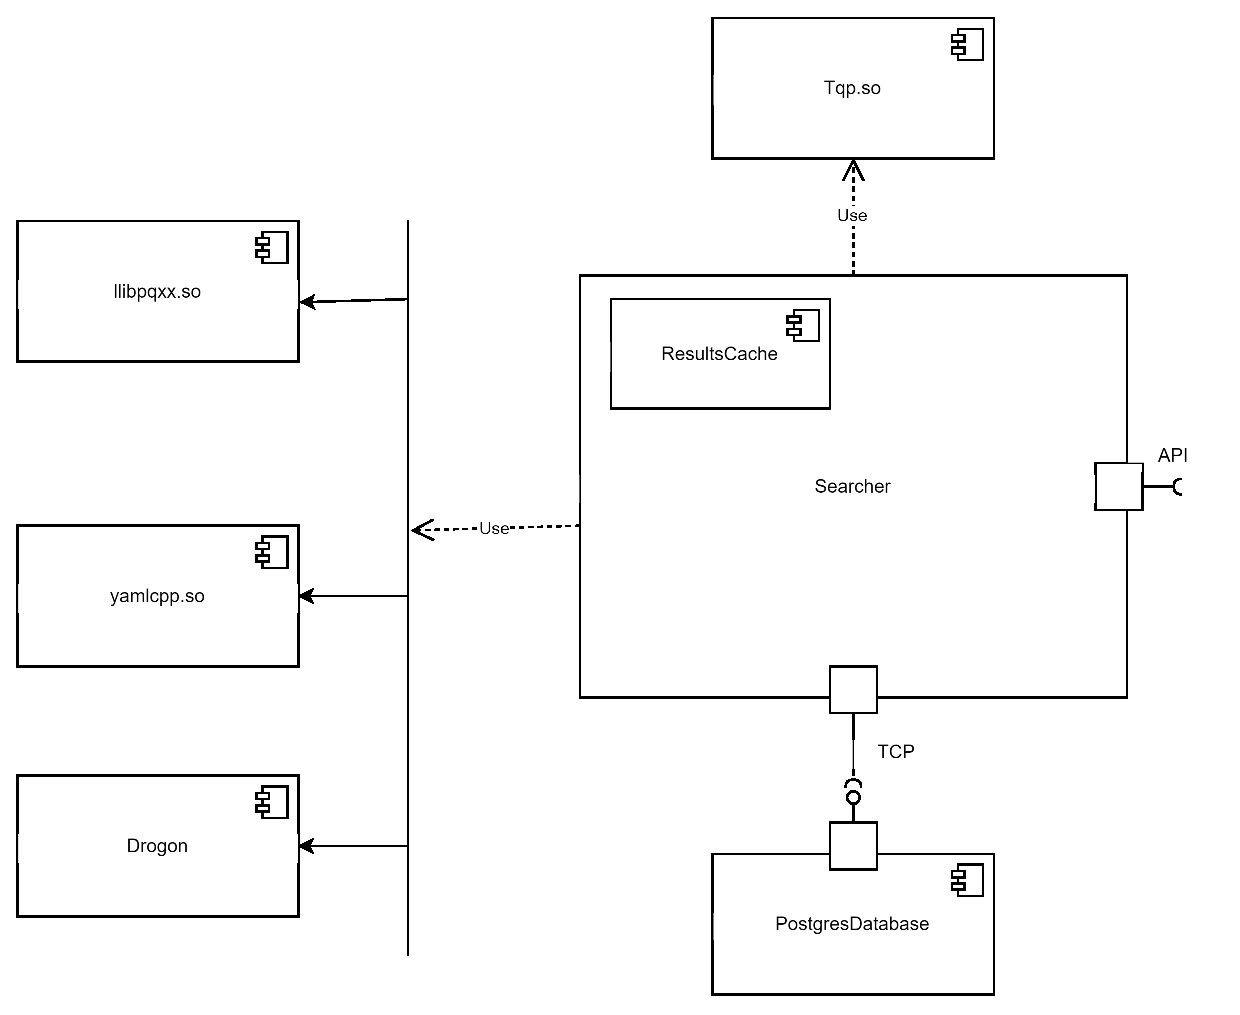
\includegraphics[width=1\linewidth]{robot/diagram_components}}
\caption{Диаграмма компонентов поискового робота}
\label{robot/diagram_components:image}
\end{figure}

\subsubsection{Описание базы данных}

На рисунке 3.2 представлена ER-диаграмма базы данных поискового робота.

\begin{figure}
\center{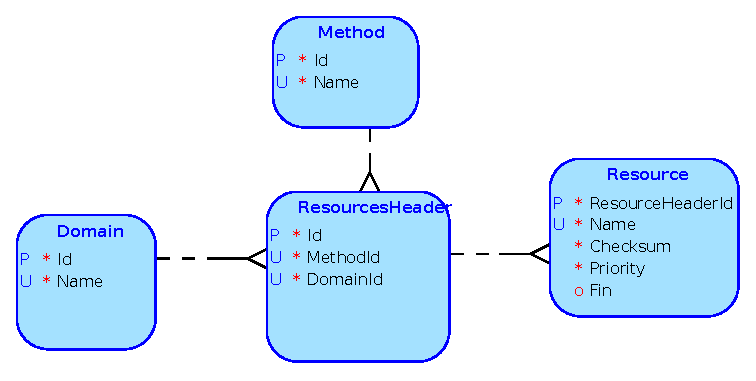
\includegraphics[width=1\linewidth]{robot/robot_db}}
\caption{ER-диаграмма базы данных поискового робота}
\label{robot/robot_db:image}
\end{figure}

\subsubsection{Описание потоков данных}

На рисунках 3.3 - 3.4 представлены диаграммы потоков данных для главного и подчиненного узлов системы соответственно.

\begin{figure}
\center{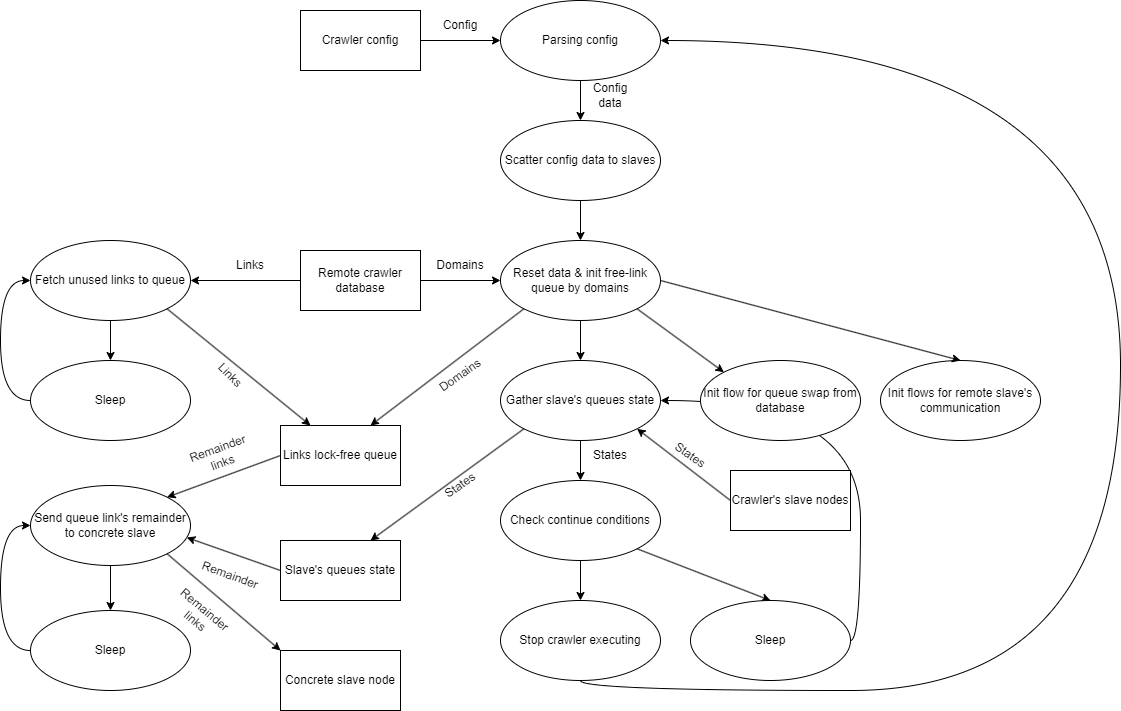
\includegraphics[width=1\linewidth]{robot/diagram_dataflow_master}}
\caption{Диаграмма потоков данных для главного узла}
\label{robot/diagram_dataflow_master:image}
\end{figure}

\begin{figure}
\center{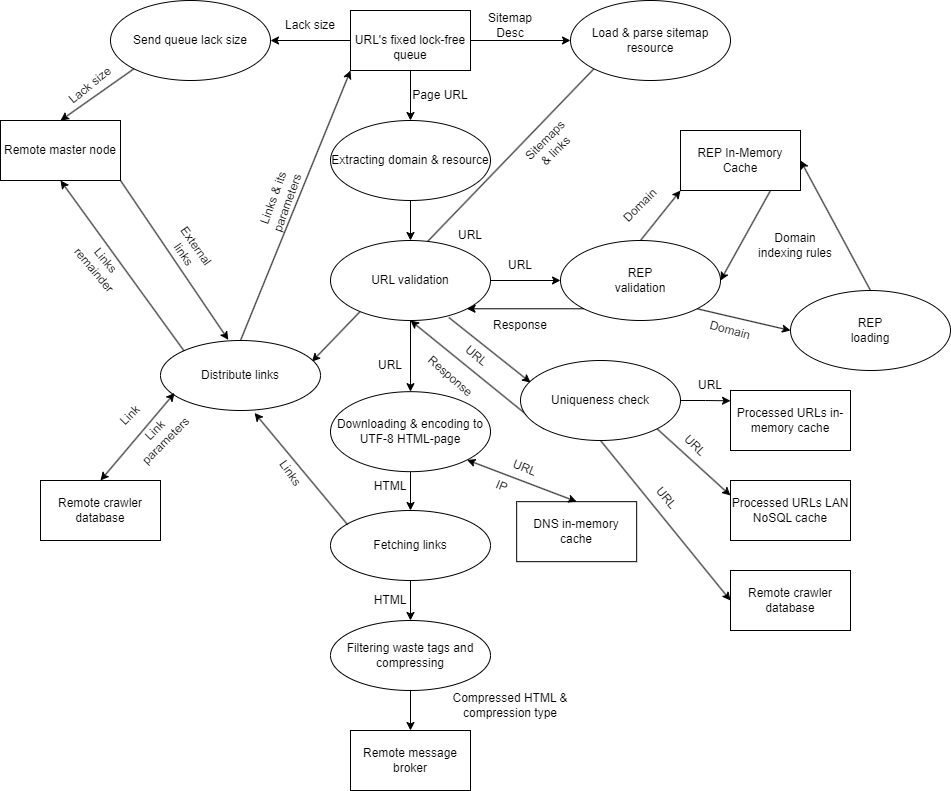
\includegraphics[width=1\linewidth]{robot/diagram_dataflow_slave}}
\caption{Диаграмма потоков данных для подчиненного узла}
\label{robot/diagram_dataflow_slave:image}
\end{figure}

\subsubsection{Описание концептуальных классов}

На рисунках 3.5 - 3.6 представлены диаграммы концептуальных классов для главного и подчиненного узлов системы соответственно.

\begin{figure}
\center{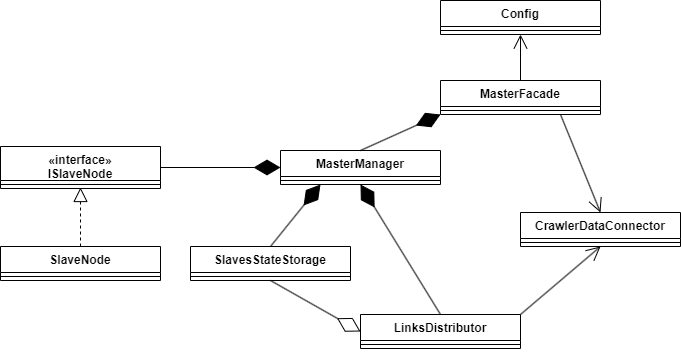
\includegraphics[width=1\linewidth]{robot/diagram_master_classes}}
\caption{Диаграмма концептуальных классов для главного узла}
\label{robot/diagram_master_classes:image}
\end{figure}

\begin{figure}
\center{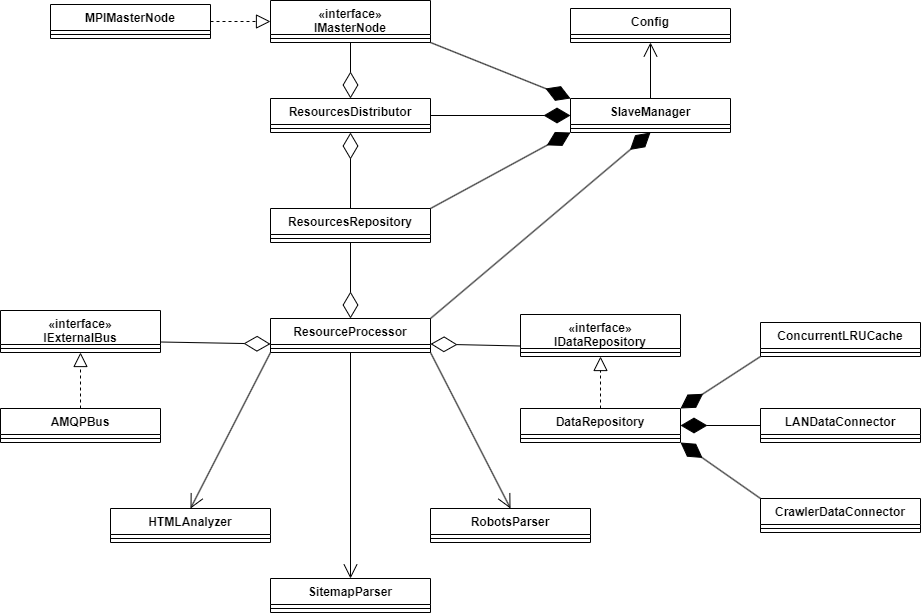
\includegraphics[width=1\linewidth]{robot/diagram_slave_classes}}
\caption{Диаграмма концептуальных классов для подчиненного узла}
\label{robot/diagram_slave_classe:image}
\end{figure}
